\chapter{Présentation de l'environnement de travail}
Dans le cadre de ce stage j'ai eu l'occasion de travailler une plusieurs technologie, beaucoup d'entre elles m'était inconnue. Ainsi, je vais expliciter les différentes technologies sur lesquelles j'ai travaillé.

\section{Gstreamer}
\label{gstreamer}
GStreamer est un framework multimédia sous licence libre publié pour la première fois le 31 octobre 1999. Il est écrit en C et est initialement pensé pour être une solution concurrente à Quicktime et Direct Show sur GNU/Linux. Aujourd'hui, GStreamer est disponible pour de nombreux systèmes d'exploitation (GNU/Linux, Solaris, BSD, Android, OS X, ios, Windows, OS/400). De plus, des bindings existent pour utiliser GStreamer dans une multitude de langages de programmation en plus du C (C++, Java, Python, Vala etc.
\begin{figure}[!h]
  \centering
  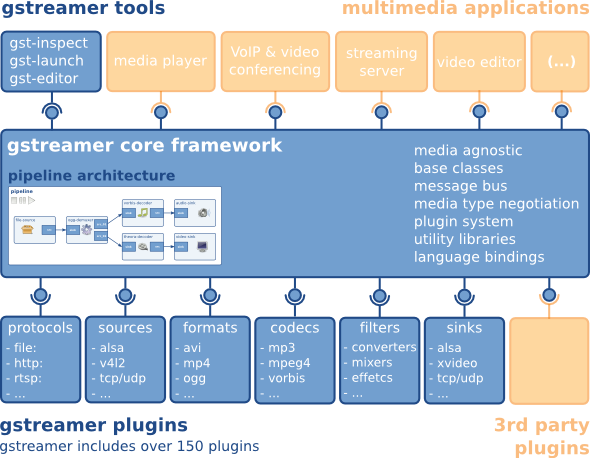
\includegraphics[scale=0.7]{figures/gstreamer-overview}
  \caption{schéma de l'architecture de Gstreamer}
\end{figure}


\subsection{Principes techniques}
\label{principe_gst}
GStreamer est basé sur un système de pipeline. Différents éléments sont connectés entre eux par des tuyaux (pipe). Chaque élément possède des "pads" servant à les connecter aux autres. Ces pads peuvent être soit des entrées (sink) soit des sorties (source).Exemple de pipeline GStreamer :ce pipeline lit un fichier *. Ogg, en sépare les pistes et décode sa piste audio et la décode pour ensuite la jouer.
\begin{figure}[!h]
  \centering
  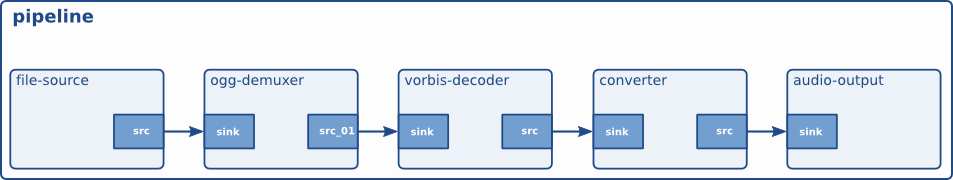
\includegraphics[scale=0.5]{figures/pipeline_ogg}
  \caption{Une pipeline gstreamer pour lire un fichier .ogg puis decode en vorbis}
\end{figure}

Une autre notion importante de GStreamer est celle de « capabilities » (capacités) ou «caps». Il s'agit d'une liste de formats et propriétés d’un flux qu'un élément peut accepter sur un pad. Par exemple, un élément acceptant uniquement un format "vidéo/x-raw" au framerate 24/1 (24 images par seconde) ne pourra pas recevoir d'autres flux (format ou framerate différent). Ainsi les caps peuvent imposer un format, une résolution, un framerate, etc. Ce sont eux qui sont utilisés par GStreamer pour négocier la connexion entre deux éléments et choisir le type de flux qui sera utilisé (si les caps sont compatibles pour au moins un type de flux, sinon la négociation échoue).

\begin{figure}[!h]
  \centering
  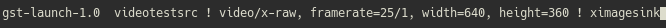
\includegraphics[scale=0.9]{figures/caps_negociation}
  \caption{pipeline avec négociation de caps}
\end{figure}

\subsection{Présentation des composants Gstreamer}
Le framework Gstreamer offre plusieurs types d'éléments, ou "plugins", afin d'effectuer des tâches différentes. Gstreamer fourni plus de 200 plugins diffèrents. Ainsi, ils permettent :\begin{itemize}[label=$\bullet$]
 \item la manipulation d’objet multimédia
 \item gestions des entrées audio/vidéo (caméra/flux réseau)
 \item gestion des protocoles réseaux
 \item gestion des filtres
 \item gestion des sorties
\end{itemize}

Lors de ce stage, j'ai particulièrement travaillé avec deux types d'élément, les multiplexeurs (ou "muxers") et les démultiplexeurs (ou " demuxers"). Les muxers sont d'élement "N-to-1" qui prennent N flux en entrée puis les "entrelacent" en un seul. Particulièrement utiles lorsque l'on voudra muxer le flux vidéo avec la métadonnée.Les démuxers font l'exact inverse, ainsi, ils prennent un flux "entrelacé" puis en fournir N.


\subsubsection{3.2.1.2 Débogage}
GStreamer possède des outils de débogage très utiles qui m'ont servi tout au long du stage. Le premier est GST\_DEBUG. Il s'agit d'une variable d’environnement qui peut-être initialisée avec une valeur de 1 à 9 permettant d'afficher plus ou moins d'informations sur le déroulement des actions initiées par GStreamer.L'autre outil est un générateur de fichier *. dot permettant de générer une représentation graphique de la pipeline. Cela permet de vérifier que la pipeline obtenu par le programme est bien celle souhaitée lors de la conception et permet de repérer simplement et rapidement certaines erreurs


\section{OpenCV}
Le projet contient des briques algorithmiques fonctionnant grâce à la bibliothèque OpenCV. OpenCV (pour open computer Vision) est une bibliothèque graphique libre, initialement développée par Intel, spécialisée dans le traitement d'images en temps réel. La société de robotique Willow Garage et la société ItSeez se sont succédées au support de cette bibliothèque, Depuis 2016 et le rachat d'ItSeez par Intel, le support est de nouveau assuré par Intel.


\section{Protobuf }
Protobuf ou "Protocol Buffers" sont un mécanisme flexible, efficace et automatisé pour sérialiser des données structurées - pensez XML, mais plus petit, plus rapide et plus simple. Vous définissez comment vous souhaitez que vos données soient structurées une fois, vous pouvez utiliser un code source généré spécialement pour écrire et lire facilement vos données structurées vers et à partir d'une variété de flux de données et en utilisant diverses langues. Vous pouvez même mettre à jour votre structure de données sans rompre les programmes déployés qui sont compilés par rapport au format.

\begin{lstlisting}[language=protobuf2,style=protobuf , frame=single,caption=modèle pour la structure d'un message,label=proto1]

 message Person {
  required string name = 1;
  required int32 id = 2;
  optional string email = 3;

  enum PhoneType {
    MOBILE = 0;
    HOME = 1;
    WORK = 2;
  }

  message PhoneNumber {
    required string number = 1;
    optional PhoneType type = 2 [default = HOME];
  }

  repeated PhoneNumber phone = 4;
}
\end{lstlisting}

C'est à l'aide de cette technique que nous formattons les métadonnées générées par les algorithmes de traitement d'images afin de les "muxer" avec le flux vidéo.

\section{Outils de provisionnement}

\subsection{Vagrant}
Vagrant est un outil de création et de gestion d'environnements de machines virtuelles. Il est un outil qui permet de démarrer des machines virtuelles avec une configuration donnée. Un très bon moyen de mettre au point et de diffuser des environnements de travail, et ce, de manière reproductible. Vagrant permet donc d'éviter le syndrome « works on my machine ».Plusieurs cas d'usage sont possibles. Le plus courant est celui de faire concevoir un environnement de développement à partir de zéros . Ensuite, à partir d'un VagrantFile\footnote{fichier de configuration de vagrant.} il suffit de saisir "vagrant up" et on dispose d'un environnement de développement.

\subsection{Ansible}
Écrit en Python, Ansible est un outil Open Source qui permet l’automatisation de tâches. Grâce à lui, nous gérons nos configurations de VM plus facilement, et de façon automatique grâce à l’exécution de taches sur des groupes d’hôtes. Il n’utilise pas de client, d’agent, sur les hôtes clients mais nécessite uniquement une partie serveur Ansible, forcément sous Linux. Par ailleurs, Ansible peut éventuellement être utilisé à des fins de contrôle, par exemple pour s’assurer que certains services soient exécutés sur un groupe de machine. Sachant qu’il est possible de développer ses propres tâches grâce aux langages YAML.



